\documentclass{article}
\usepackage{graphicx} % Required for inserting images
\usepackage{amsmath}
\usepackage{amsfonts}
\usepackage{comment}
\usepackage{microtype}
\usepackage{bm}
\usepackage{multicol}

\usepackage{mathtools}
\DeclarePairedDelimiter\bra{\langle}{\rvert}
\DeclarePairedDelimiter\ket{\lvert}{\rangle}
\DeclarePairedDelimiterX\braket[2]{\langle}{\rangle}{#1\delimsize\vert\mathopen{}#2}
\newcommand*\diff{\mathop{}\!\mathrm{d}}
\DeclarePairedDelimiterX\expval[3]{\langle}{\rangle}%
{#1\delimsize\vert\mathopen{}#2\delimsize\vert\mathopen{}#3}
\newcommand\HF{\ensuremath{\mathrm{HF}}}

\usepackage{hyperref}
\usepackage{xcolor}
\hypersetup{ % this is just my personal choice, feel free to change things
    colorlinks,
    linkcolor={red!50!black},
    citecolor={blue!50!black},
    urlcolor={blue!80!black},
}

\usepackage{simpler-wick}

\usepackage{enumerate}
\usepackage[shortlabels]{enumitem}
\usepackage{booktabs}
\usepackage{tikz}

\renewcommand\thesection{Exercise \alph{section})}  % chktex 9 % chktex 10 % tex-fmt: skip
\renewcommand\thesubsection{Solution} % tex-fmt: skip
\renewcommand\thesubsubsection{\arabic{subsection}.\arabic{subsubsection})} % chktex 9 % chktex 10 % tex-fmt: skip

\title{
    Second midterm FYS4480\\
    Quantum mechanics for many-particle systems
}
\author{August Femtehjell \& Oskar Idland}
\date{November 2024}

\begin{document}

\maketitle

\section*{Introduction}
We present a simplified Hamiltonian consisting of an unperturbed Hamiltonian and a so-called pairing interaction term.
It is a model which to a large extent mimicks some central features of atomic nuclei, certain atoms and systems which exhibit superfluiditity or superconductivity.
To study this system, we will use a mix of many-body perturbation theory (MBPT), Hartree-Fock (HF) theory and full configuration interaction (FCI) theory.
The latter will also provide us with the exact answer.
When setting up the Hamiltonian matrix you will need to solve an eigenvalue problem.

We define first the Hamiltonian, with a definition of the model space and the single-particle basis.
Thereafter, we present the various exercises.

The Hamiltonian acting in the complete Hilbert space (usually infinite dimensional) consists of an unperturbed one-body part, $\hat{H}_0$, and a perturbation $\hat{V}$.
We limit ourselves to at most two-body interactions, our Hamiltonian is then represented by the following operators
\begin{equation*}
    \hat{H} = \sum_{\alpha\beta} \langle \alpha \lvert h_0 \rvert \beta \rangle a_{\alpha}^{\dagger} a_{\beta}
    + \frac{1}{4} \sum_{\alpha\beta\gamma\delta} \langle
    \alpha \beta \lvert V \rvert \gamma\delta
    \rangle
    a_{\alpha}^{\dagger} a_{\beta}^{\dagger} a_{\delta} a_{\gamma},
\end{equation*}
where $a_{\alpha}^{\dagger}$ and $a_{\alpha}$ etc.~are standard fermion creation and annihilation operators, respectively, and
$\alpha\beta\gamma\delta$ represent all possible single-particle quantum numbers.
The full single-particle space is defined by the completeness relation $\hat{{\bf 1}} = \sum_{\alpha
= 1}^{\infty} \lvert \alpha \rangle \langle \alpha \rvert$.
In our calculations we will let the single-particle states $\lvert \alpha \rangle$ be eigenfunctions of the one-particle operator $\hat{h}_0$.
Note that the two-body part of the Hamiltonian contains anti-symmetrized matrix elements.

The above Hamiltonian acts in turn on various many-body Slater determinants constructed from the single-basis defined by the one-body operator $\hat{h}_0$.
As an example, the two-particle model space $\mathcal{P}$ is defined by an operator
\begin{equation*}
    \hat{P} = \sum_{\alpha\beta =1}^{m} \lvert \alpha\beta \rangle \langle \alpha\beta \rvert,
\end{equation*}
where we assume that $m = \dim(\mathcal{P})$ and the full space is defined by
\begin{equation*}
    \hat{P}+\hat{Q}=\hat{{\bf 1}},
\end{equation*}
with the projection operator
\begin{equation*}
    \hat{Q} = \sum_{\alpha\beta =m+1}^{\infty} \lvert \alpha\beta \rangle \langle \alpha\beta \rvert,
\end{equation*}
being the complement of $\hat{P}$.

Our specific model consists of $N$ doubly-degenerate and equally spaced single-particle levels labelled by $p = 1, 2, \ldots$ and spin $\sigma = \pm 1$.
These states are schematically portrayed in Fig.~\ref{fig:schematic}.
The first two single-particle levels define a possible model space, indicated by the label $\mathcal{P}$.
The remaining states span the excluded space $\mathcal{Q}$.

We write the Hamiltonian as
\begin{equation*}
    \hat{H} = \hat{H}_0 + \hat{V},
\end{equation*}
where
\begin{equation*}
    \hat{H}_0 = \xi \sum_{p\sigma}(p - 1) a_{p\sigma}^{\dagger} a_{p\sigma}
\end{equation*}
and
\begin{equation*}
    \hat{V} = -\frac{1}{2} g \sum_{pq} a^{\dagger}_{p+} a^{\dagger}_{p-} a_{q-} a_{q+}.
\end{equation*}
Here, $H_0$ is the unperturbed Hamiltonian with a spacing between successive single-particle states given by $\xi$, which we will set to a constant value $\xi=1$ without loss of generality.
The two-body operator $\hat{V}$ has one term only.
It represents the pairing contribution and carries a constant strength $g$.

The indices $\sigma = \pm$ represent the two possible spin values.
The interaction can only couple pairs and excites therefore only two particles at the time, as indicated by the rightmost four-particle state in Fig.~\ref{fig:schematic}.
There one of the pairs is excited to the state with $p = 9$ and the other to the state $p = 7$.
The two middle possibilities are not possible with the present model.
We label single-particle states within the model space as hole-states.
The single-particle states outside the model space are then particle states.

In our model we have kept both the interaction strength and the single-particle level as constants.
In a realistic system like an atom or the atomic nucleus this is not the case.

\begin{figure}[htbp]
    \centering
    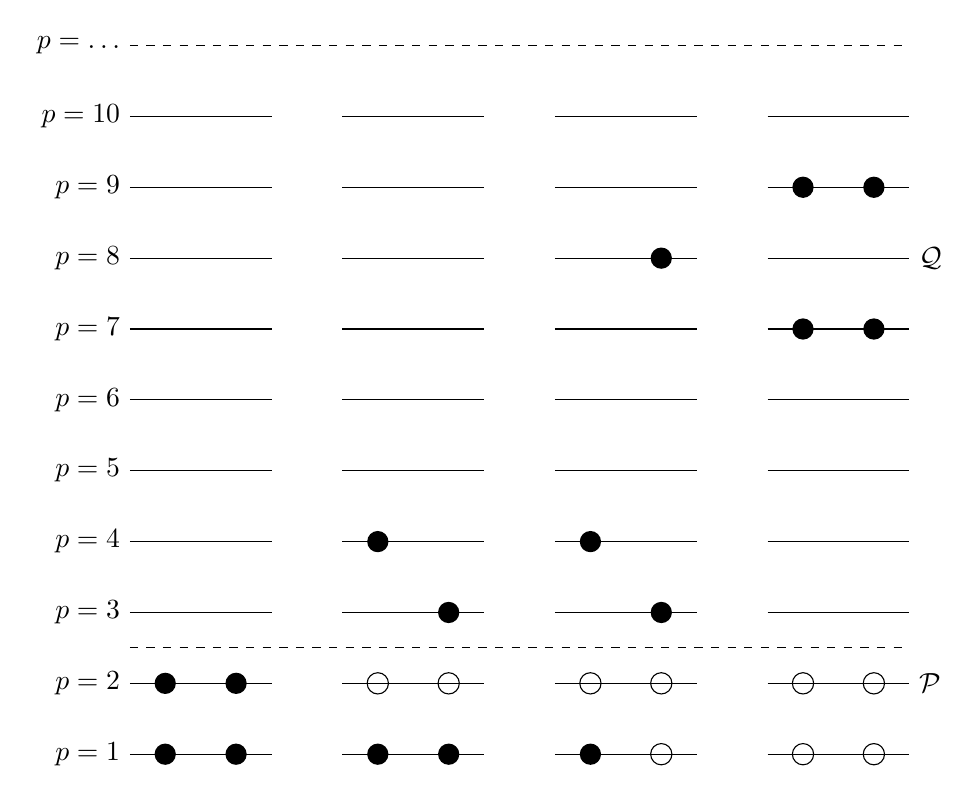
\begin{tikzpicture}[scale=0.9]
        % Draw lines
        \foreach \y in {1,2,...,10} {
            \draw (0, \y) -- (2, \y);
            \draw (3, \y) -- (5, \y);
            \draw (6, \y) -- (8, \y);
            \draw (9, \y) -- (11, \y);
            % \draw (12, \y) -- (14, \y);
        }
        % Draw additional dashed lines
        \draw[dashed] (0, 2.5) -- (11, 2.5);
        \draw[dashed] (0, 11) -- (11, 11);

        % Labels on the left
        \foreach \y/\label in {1/$p=1$, 2/$p=2$, 3/$p=3$, 4/$p=4$, 5/$p=5$, 6/$p=6$, 7/$p=7$, 8/$p=8$, 9/$p=9$, 10/$p=10$, 11/$p=\ldots$} {
            \node[left] at (0, \y) {\label};
        }

        % Labels on the right
        \node[right] at (11, 8) {$\mathcal{Q}$};
        \node[right] at (11, 2) {$\mathcal{P}$};

        % First 4-particle state
        \foreach \x/\y in {0.5/1, 0.5/2, 1.5/1, 1.5/2} {
            \fill (\x, \y) circle (0.15);
        }

        % Second 4-particle state
        \foreach \x/\y in {3.5/1, 4.5/1, 3.5/4, 4.5/3} {
            \fill (\x, \y) circle (0.15);
        }
        \foreach \x/\y in {3.5/2, 4.5/2} {
            \draw (\x, \y) circle (0.15);
        }

        % Third 4-particle state
        \foreach \x/\y in {6.5/1, 7.5/3, 6.5/4, 7.5/8} {
            \fill (\x, \y) circle (0.15);
        }
        \foreach \x/\y in {7.5/1, 6.5/2, 7.5/2} {
            \draw (\x, \y) circle (0.15);
        }

        % Fourth 4-particle state
        \foreach \x/\y in {9.5/7, 10.5/7, 9.5/9, 10.5/9} {
            \fill (\x, \y) circle (0.15);
        }
        \foreach \x/\y in {9.5/1, 10.5/1, 9.5/2, 10.5/2} {
            \draw (\x, \y) circle (0.15);
        }
    \end{tikzpicture}
    \caption{
        Schematic plot of the possible single-particle levels with double degeneracy.
        The filled circles indicate occupied particle states while the empty circles represent vacant particle (hole) states.
        The spacing between each level $p$ is constant in this picture.
        The first two single-particle levels define our possible model space, indicated by the label $\mathcal{P}$.
        The remaining states span the excluded space $\mathcal{Q}$.
        The first state to the left represents a possible ground state representation for a four-fermion system.
        In the second state to the left, one pair is broken.
        This possibility is however not included in our interaction.\label{fig:schematic}
    }
\end{figure}

\newpage
\section{}
We start with the helium atom and define our single-particle Hilbert
space to consist of the single-particle orbits \(1s\), \(2s\) and \(3s\),
with their corresponding spin degeneracies.

Set up the ansatz for the ground state \(\ket*{c} = \ket*{\Phi_0}\) in second quantization.
Define the second quantization and define a table of single-particle states.
Construct thereafter all possible one-particle-one-hole
excitations \(\ket*{\Phi_i^a}\) where \(i\) refer to levels below the Fermi level (define this level) and \(a\) refers to particle states.
Define particles and holes.
The Slater determinants have to be written in terms of the respective creation and annihilation operators.
The states you construct should all have total spin projection \(M_S=0\).
Construct also all possible two-particle-two-hole states \(\ket*{\Phi_{ij}^{ab}}\) in a second quantization
representation.

\subsection{}
We define the Fermi level as \(1s\), such that the ground state is given by
\begin{equation}
    \ket*{\Phi_0} = \ket*{c} = a_{1\sigma_1}^\dagger a_{1\sigma_2}^\dagger \ket*{0},
\end{equation}
where we define $\sigma_1 = \ \uparrow \ = +1/2$ and $\sigma_2 = \ \downarrow \ = -1/2$.
Here, we define particles as electrons (?) above the Fermi level, and holes as the lack of electrons in slots below the Fermi level.

In order to have a one-particle-one-hole excitation, the spin in the hole and particle states must match.
All possible one-particle-one-hole (1p1h) excitations are then
\begin{align*}
    \ket*{\Phi_{1\sigma_1}^{2\sigma_1}} &= a_{2\sigma_1}^\dagger a_{1\sigma_1} \ket*{\Phi_0}, &
    \ket*{\Phi_{1\sigma_1}^{3\sigma_1}} &= a_{3\sigma_1}^\dagger a_{1\sigma_1} \ket*{\Phi_0}, \\
    \ket*{\Phi_{1\sigma_2}^{2\sigma_2}} &= a_{2\sigma_2}^\dagger a_{1\sigma_2} \ket*{\Phi_0}, &
    \ket*{\Phi_{1\sigma_2}^{3\sigma_2}} &= a_{3\sigma_2}^\dagger a_{1\sigma_2} \ket*{\Phi_0},
\end{align*}
where we always excite a particle from the $1s$ state, to the higher states, with the same spin such that $M_S = 0$.

For the possible two-particle-two-hole (2p2h) excitations $\ket*{\Phi_{ij}^{ab}}$, we have that both electrons below the Fermi level excite, and that the particles above the Fermi level have opposite spins.
We then have that the possible configurations are
\begin{align*}
    \ket*{\Phi_{1\sigma_1, 1\sigma_2}^{2\sigma_1, 2\sigma_2}} &= a_{2\sigma_1}^\dagger a_{2\sigma_2}^\dagger a_{1\sigma_2} a_{1\sigma_1} \ket*{\Phi_0}, &
    \ket*{\Phi_{1\sigma_1, 1\sigma_2}^{2\sigma_1, 3\sigma_2}} &= a_{2\sigma_1}^\dagger a_{3\sigma_2}^\dagger a_{1\sigma_2} a_{1\sigma_1} \ket*{\Phi_0}, \\
    \ket*{\Phi_{1\sigma_1, 1\sigma_2}^{3\sigma_1, 2\sigma_2}} &= a_{3\sigma_1}^\dagger a_{2\sigma_2}^\dagger a_{1\sigma_2} a_{1\sigma_1} \ket*{\Phi_0}, &
    \ket*{\Phi_{1\sigma_1, 1\sigma_2}^{3\sigma_1, 3\sigma_2}} &= a_{3\sigma_1}^\dagger a_{3\sigma_2}^\dagger a_{1\sigma_2} a_{1\sigma_1} \ket*{\Phi_0}.
\end{align*}



\end{document} % chktex 17
